\section{Circuit}
\subsection{Data encoding}
\par In this experiment, we use fraxis encoding. Fraxis encoding is newly introduced in this research, and is very similar to angle encoding.

\subsubsection{Fraxis encoding}
\par Assume that the data $\bm{x}$ is the $2LQ$-dimensional real vector. Then, the representation of this data is done by the following circuit (Figure \ref{fig:fraxis_enco}). The number of the required qubits is $Q$. 

\begin{figure}[H]
    \centering
    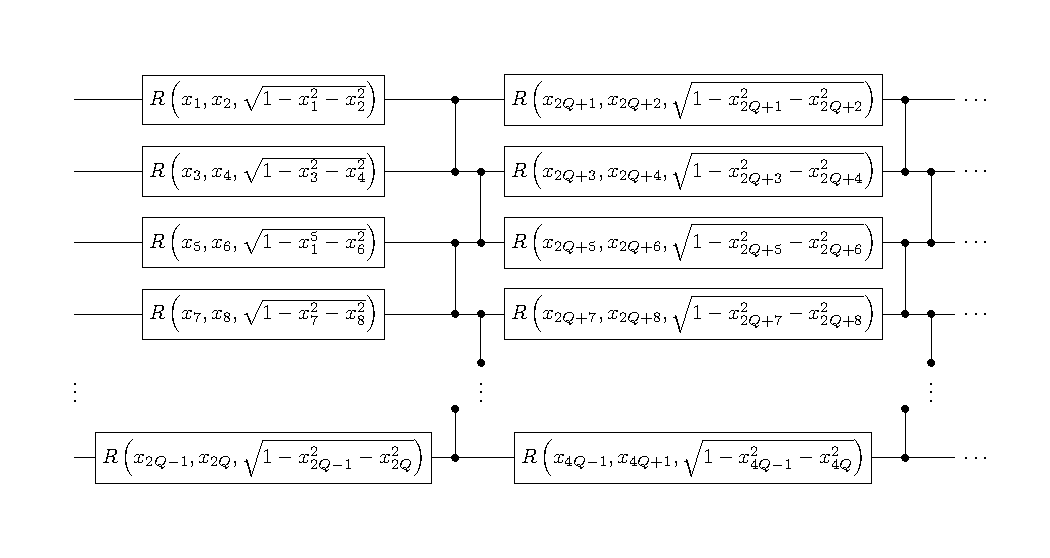
\includegraphics[keepaspectratio, scale=0.5]{experiment/figure/fraxis_enco.pdf}
    \caption{Fraxis encoding used in this research.}
    \label{fig:fraxis_enco}
\end{figure}

\par As seen above, the first $2Q$ elements are embedded into each qubit using fraxis gates, then these qubits are entangled using a CZ layer, and the next $2Q$ elements are embedded into each qubit using fraxis gates, then entangle these qubits using a CZ layer, and so on $L$ times. When the dimension of the data is not $2LQ$, we place elements from the beginning into the fraxis encoding, and the remaining elements are put in fraxis gate's parameters and appended to the end of fraxis encoding.

\subsection{Overall circuit}
Here we define the fraxis layer as shown in Figure \ref{fig:ansatz}.
\begin{figure}[H]
    \centering
    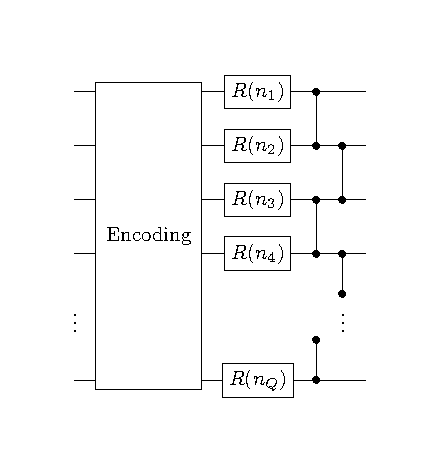
\includegraphics[keepaspectratio, scale=1]{experiment/figure/layer.pdf}
    \caption{Fraxis layer on $Q$ qubits.}
    \label{fig:ansatz}
\end{figure}
After encoding the data, fraxis gates is applied to all bits and finally CZ gates are alternately applied.
\par The entire circuit repeats this fraxis layer $L$ times, as shown in the figure \ref{fig:whole}.
\begin{figure}[H]
    \centering
    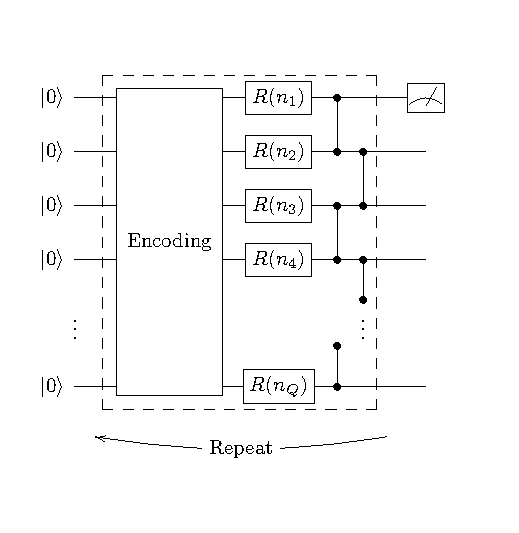
\includegraphics[keepaspectratio, scale=1]{experiment/figure/whole.pdf}
    \caption{Overall circuit on $Q$ qubits.}
    \label{fig:whole}
\end{figure}

\par In this experiments, we initialize all the fraxis gates' parameters to $\bm{n}=(0,0,1)^\top$. The order of the updating of the parameters are cyclically fixed. That means, from the fraxis gate of the first qubit of the first layer, then the second qubit of the first layer, and so on to the final qubit of the first layer, and after the updating of the first layer, then the second layer, the third layer, and so on.